\documentclass[runningheads]{llncs}
% Packages
\usepackage{graphicx}
\usepackage{url}

\begin{document}

\title{Process Discovery using Big Data stack - Implementing the Alpha Algorithm with Map-Reduce}
\subtitle{Design Specification Document}

\author{Martin Hashem, Xiangan Chen}

\institute{
\today \\
RWTH Aachen \\
}
% End of title
\maketitle

\section{Introduction}
Process mining is an approach to extract process models from event logs. Since the distributed nature of modern information systems, event logs are likely to be distributed among different physical machines. Map-Reduce is a scalable approach for efficient computations on distributed data. In this Python application we will present the main idea of a Map-Reduce implementation of the Alpha process mining algorithm, to take advantage of the scalability of the Map-Reduce approach.\\

\noindent
To fulfill the shortcoming in the current process mining technology, this project aims to build a new python-based web service, that integrates the big data capabilities of the Hadoop system into the process mining framework pm4py.\\

\noindent
This document is presented for our shareholders of the project.

\noindent
Within our project we mostly apply well-established open source applications, which includes the following tools with version numbers:

\begin{itemize}
	\item[\Large $\cdot$]   Python 3.6 as back end programming language
	\item[\Large $\cdot$]   pm4py 1.1.10  as process mining toolkit
	\item[\Large $\cdot$]   Flask 1.0.2 as web framework
	\item[\Large $\cdot$]   Hadoop 3.2.0 as big data processing and distributed computation framework
	\item[\Large $\cdot$]   Docker CE as deploy platform
\end{itemize}

\noindent
This very document is one of these, which will be provided to bring insights to our software development cycle:

\begin{itemize}
	\item[\Large $\cdot$]  Project initiation document
	\item[\Large $\cdot$]  Requirements analysis document
	\item[\Large $\cdot$]  Design specification document
	\item[\Large $\cdot$]  Software documentation
\end{itemize}

\section{System Overview}
The main goal of this project is to create a web application that provides calculations with the Alpha algorithm and can prepare the data using the Map-Reduce. \\

\noindent
The web service is to be accessed by a standard browser and needs to provide the following functionalities:
\begin{itemize}
	\item[\Large $\cdot$] Upload event logs in either CSV or XES format into the Hadoop system
	\item[\Large $\cdot$] Front end links to existing algorithms for further processing
	\item[\Large $\cdot$] Do Map-Reduce computations to run the alpha algorithm
	\item[\Large $\cdot$] Download the files onto local system
\end{itemize}

\section{Design Considerations}
\subsection{Assumptions and Dependencies}
For an easy deployment for our entire system, we decided to use Docker, since it also is used for the distributed filesystem Hadoop. This Module will also be conform with PM4py and will share an interface with it. For this integration the programming language will be Python and for the webframework we choose the minimal framework Flask, for a resource friendly environment. \\

\noindent
The standard setup will be a single system Hadoop node, but it can be easily changed to multiple (existing) nodes. A deploy script will be available for this in Linux (Debian, Ubuntu will be supported for sure) , and as parameters only the ip's / addresses of the nodes will be neccessary [this might be subject to change].

\subsection{General Constraints}

The deployment is set for a server of unknown size, so a general minimum will be set, and tested for the deploy. To be integratable into PM4py the language for front and back end will be Python. The front end will needed to be accessibil from a standard internet browser and multiple instances can be expected, therefore minimal framework is needed. The server backend will need to calculate the MapReduce for the eventlogs and then use the Alpha-Algorithm on the MapReduce logs. The outputted petri net is needed to be ready for further access in PM4py. It needs to be downloadable from the frontend as well.

\subsection{Goals and Guidelines}

\begin{itemize}
	\item[\Large $\cdot$] \textbf{Simple:}
	One of the main guidelines through our system design is simple. From the frontend part to the backend, from the UIs to the layout, we set the simpleness on the crucial level.\\
	\item[\Large $\cdot$] \textbf{Resource-saving:}
	The other goal of our design is resource-saving. Not only in our implement but also the outcoming software, we consume resources as little as possible, inclusive CPU computing time , storage and server occupancy.
\end{itemize}

\subsection{Development Methods}

Scrum is our first choice of development method. Since we have a small team, so an agile and intensive development method should fit us better. So instead of the classic waterfall model development, our team prefer Scrum. Scrum is a lightweight, iterative and incremental framework for managing product development. And enables our team to self-organize by encouraging physical co-location or close online collaboration of all team members, as well as daily face-to-face communication among all team members.\cite{wiki:xxx}

\section{System Architecture}
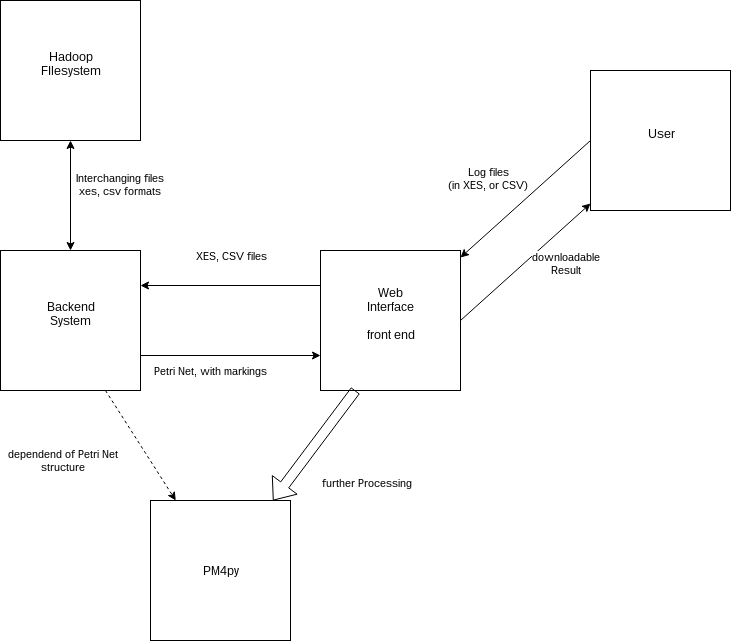
\includegraphics[scale=.35]{HighLevelDesign.png} \\ \ \\
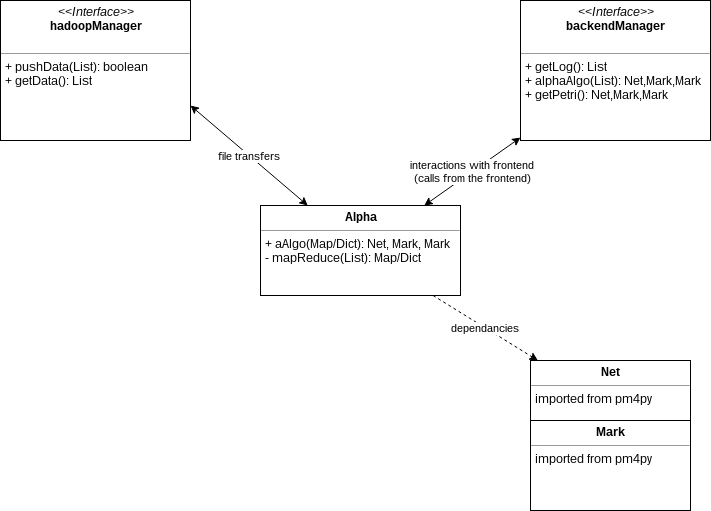
\includegraphics[scale=.35]{Backend.png} \\ \ \\
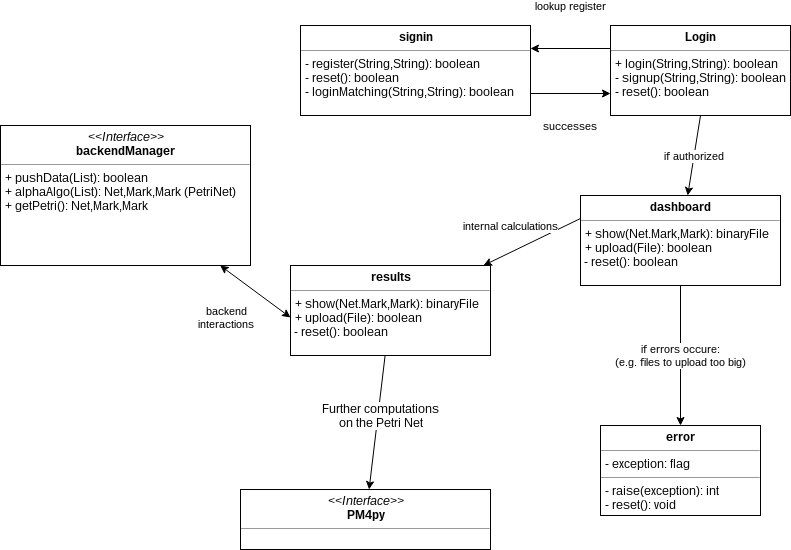
\includegraphics[scale=.35]{WebApp.png}
\section{Policies and Tactics}

\section{Detailed System Design}
\subsection{Net}
\begin{itemize}
	\item[Name:] Net
	\item[Type:] Class
	\item[Attributes:] places, transitions, arcs
	\item[Description:] Inherited Petri Nets from PM4py for further use in PM4py.
\end{itemize}
\subsection{hadoopManager}
\begin{itemize}
\item[Name:] pushData
\item[Returns:] Boolean
\item[Arguments:] List
\item[Description:] takes a list of events (from the event log) to push into the Hadoop filesystem, and returns a boolean with the success from the push.
\end{itemize}

\begin{itemize}
\item[Name:] getData
\item[Returns:] List
\item[Arguments:] -
\item[Description:] returns the entire list of saved events.
\end{itemize}

\subsection{Alpha}
\begin{itemize}
\item[Name:] mapReduce
\item[Returns:] Dict/Map
\item[Arguments:] List
\item[Description:] calculates the MapReduce of a given list of events.
\end{itemize}

\begin{itemize}
\item[Name:] aAlgo
\item[Returns:] Net, initMark, finMark
\item[Arguments:] Dict/Map
\item[Description:] Takes a MapReduced eventlog and mines the process as a Petri Net.
\end{itemize}

\subsection{backendManager}
\begin{itemize}
\item[Name:] getLog
\item[Returns:] List
\item[Arguments:] -
\item[Description:] to be called from outside the backend. Returns the log-list from the Hadoop system.
\end{itemize}
\begin{itemize}
\item[Name:] alphaAlgo
\item[Returns:] Net, initMark, finMark
\item[Arguments:] List
\item[Description:] takes a List of events and then returns the mined Perti Net. The MR will be calculated, a call for the MR-Method is not needed.
\end{itemize}

\begin{itemize}
\item[Name:] getPetri
\item[Returns:] Net, initMark, finMark
\item[Arguments:] -
\item[Description:] takes the list of events in Hadoop and calculates the Perti Net over all of them.
\end{itemize}

% Start bibliography
\bibliographystyle{alpha}
\bibliography{DesignDocument}

\end{document}
